\section{Kernel Classes}
\label{section:kernelclasses}

The BALL kernel data structures have been designed to model the problem 
domain (\ie well-known biochemical entities) as closely as possible.
Although some of the terms in biochemistry are rather fuzzy, there is a clear
hierarchical relationship (Fig.~\ref{figure:problem-domain}).
BALL tries to model this hierarchical relationship as a tree structure.
The design pattern used to implement this tree is the {\em composite
pattern}~\cite{DesignPatterns}, which is implemented in the \class{Composite}
class. Derived from \class{Composite} is the \class{AtomContainer} class, the
base class of all classes handling atoms. Also the \class{Atom} class is 
derived from \class{Composite}. The typical user will probably use only derived
classes of \class{AtomContainer}: \class{Atom} and \class{Molecule}. The kernel
classes decompose into three frameworks: the general molecular framework, the 
protein framework, and the nucleic acid framework 
(Fig.~\ref{figure:kernel-frameworks}).
Each of these frameworks contains a few classes which try to model the
respective problem domain as closely as possible. We will briefly discuss the
roles of each of these classes (Sections \ref{section:molecularframework} to
\ref{section:nucleicacidframework}) before describing some of the general 
features of the kernel classes.

By deriving all kernel classes from the common base class \class{Composite},
they share all the features implemented there. The following Section 
\ref{section:iterators} will briefly discuss some of these features.

\begin{figure}[tb]
  \centering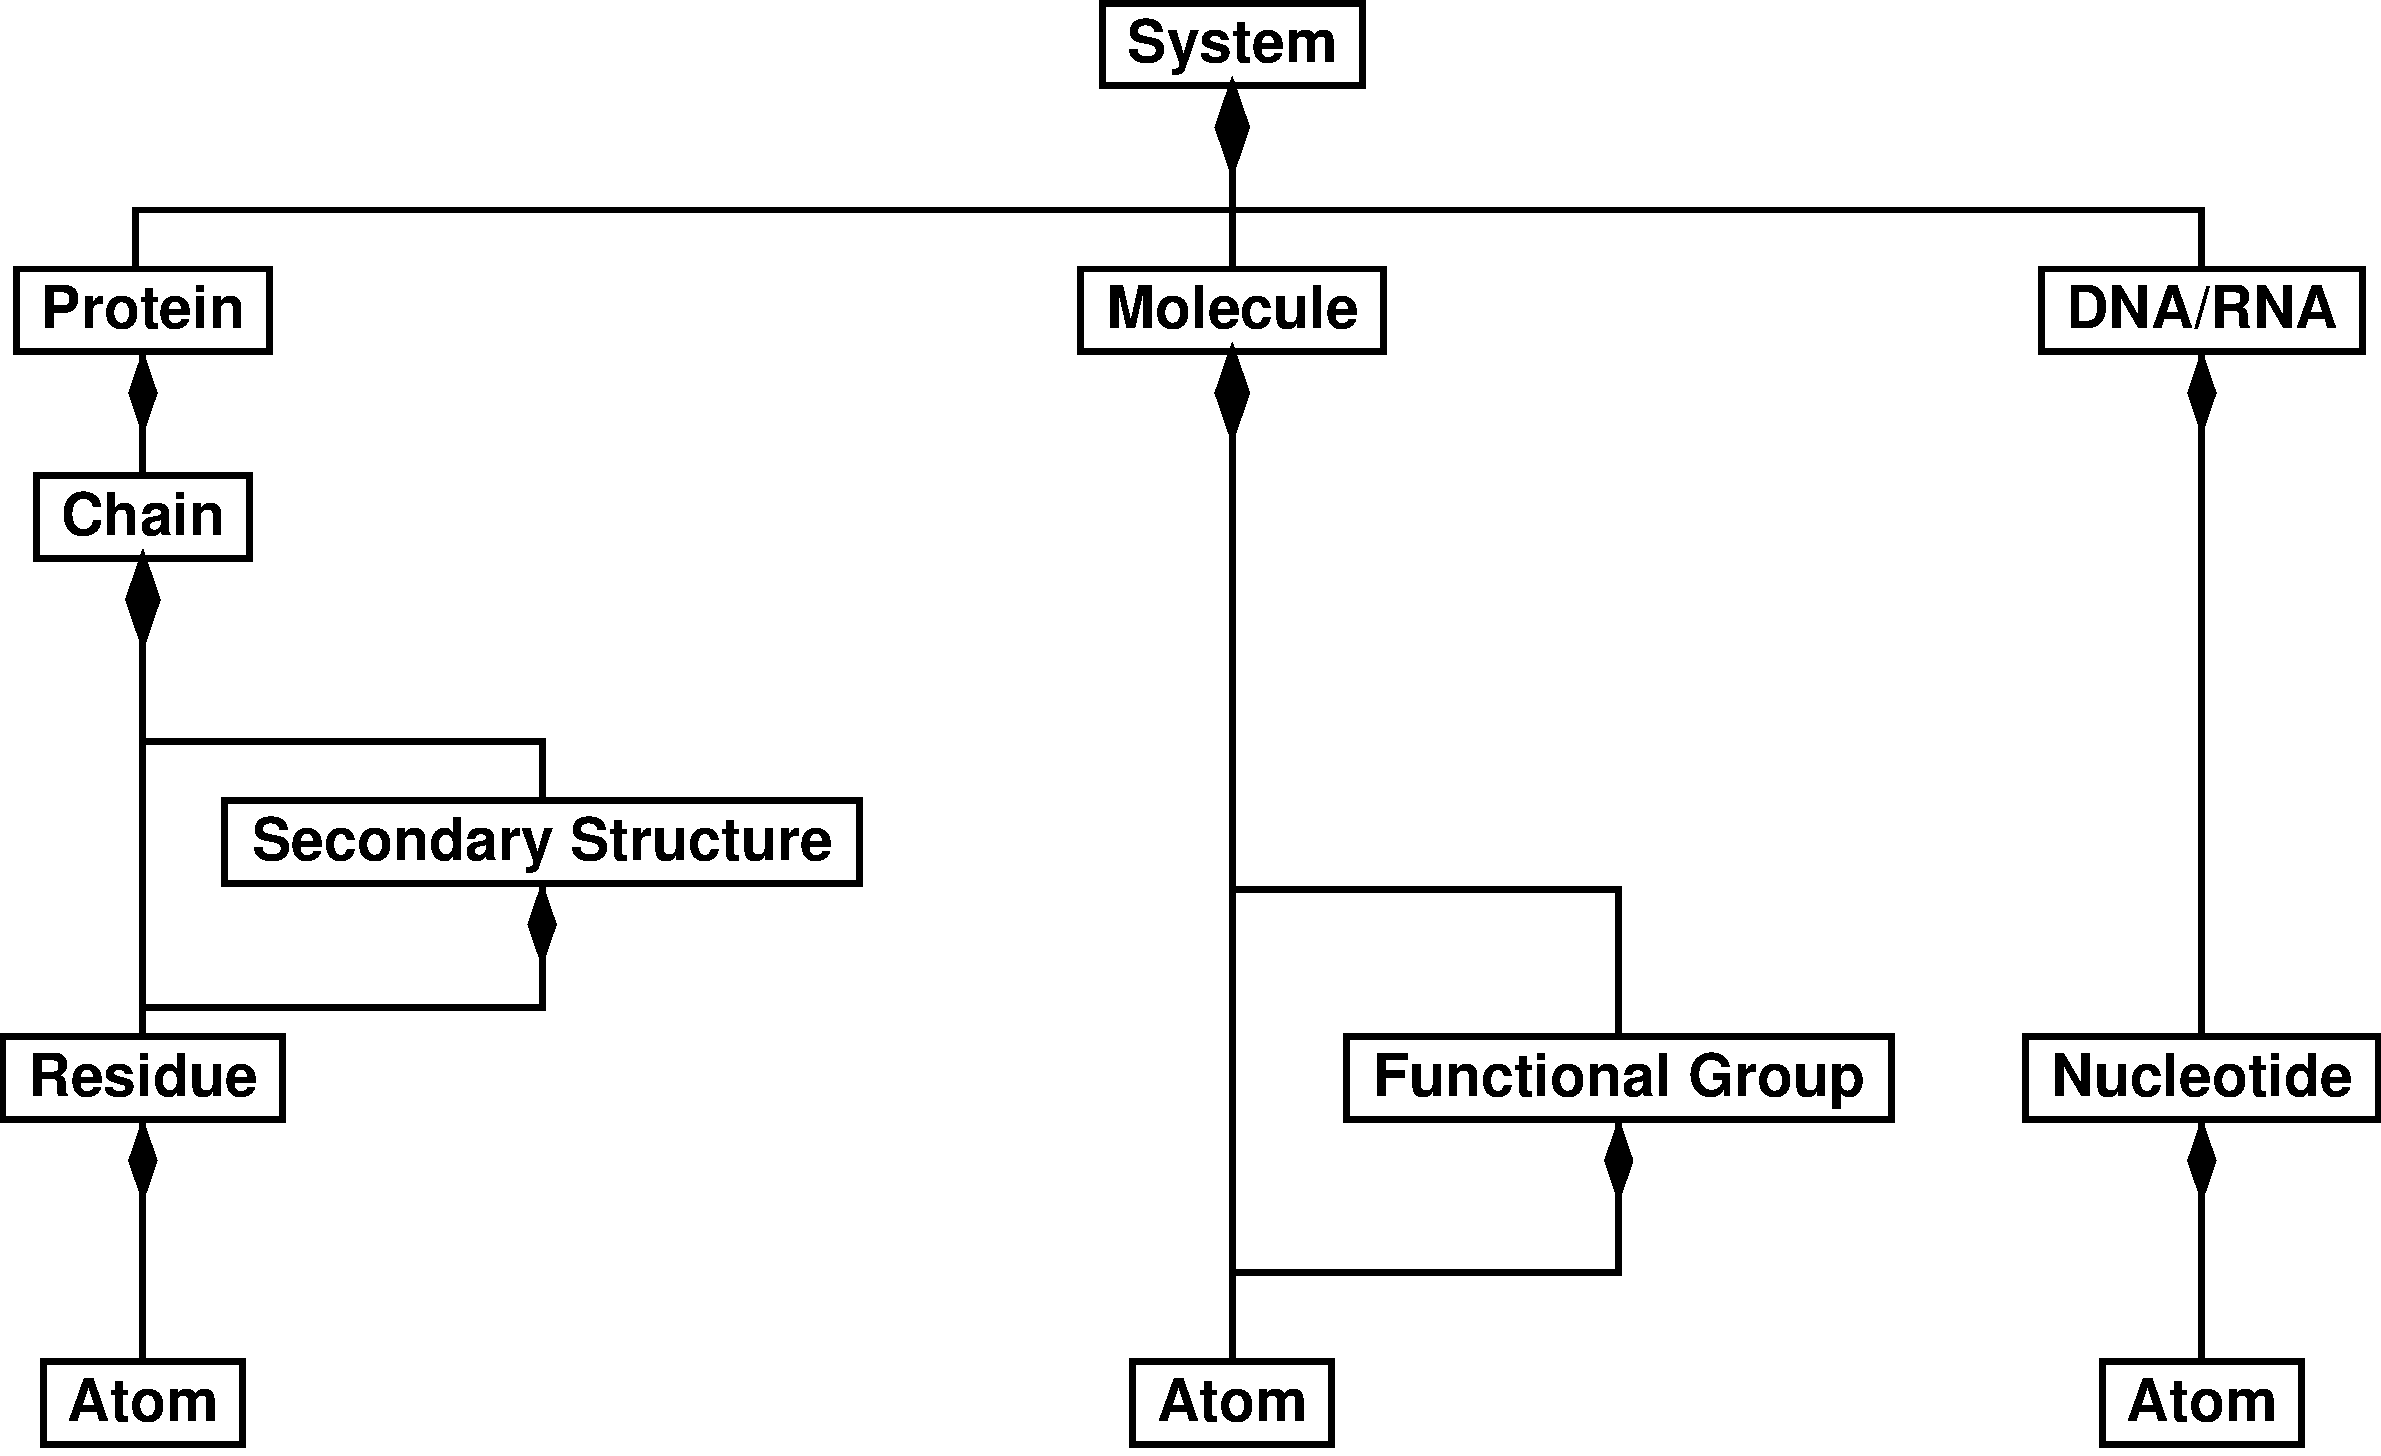
\includegraphics[width=\textwidth]{problem-domain}
  \caption{A model of the biochemical problem domain. BALL tries to model
           these entities as closely as possible with its kernel classes.}
  \label{figure:problem-domain}
\end{figure}

\begin{figure}[tb]
  \centering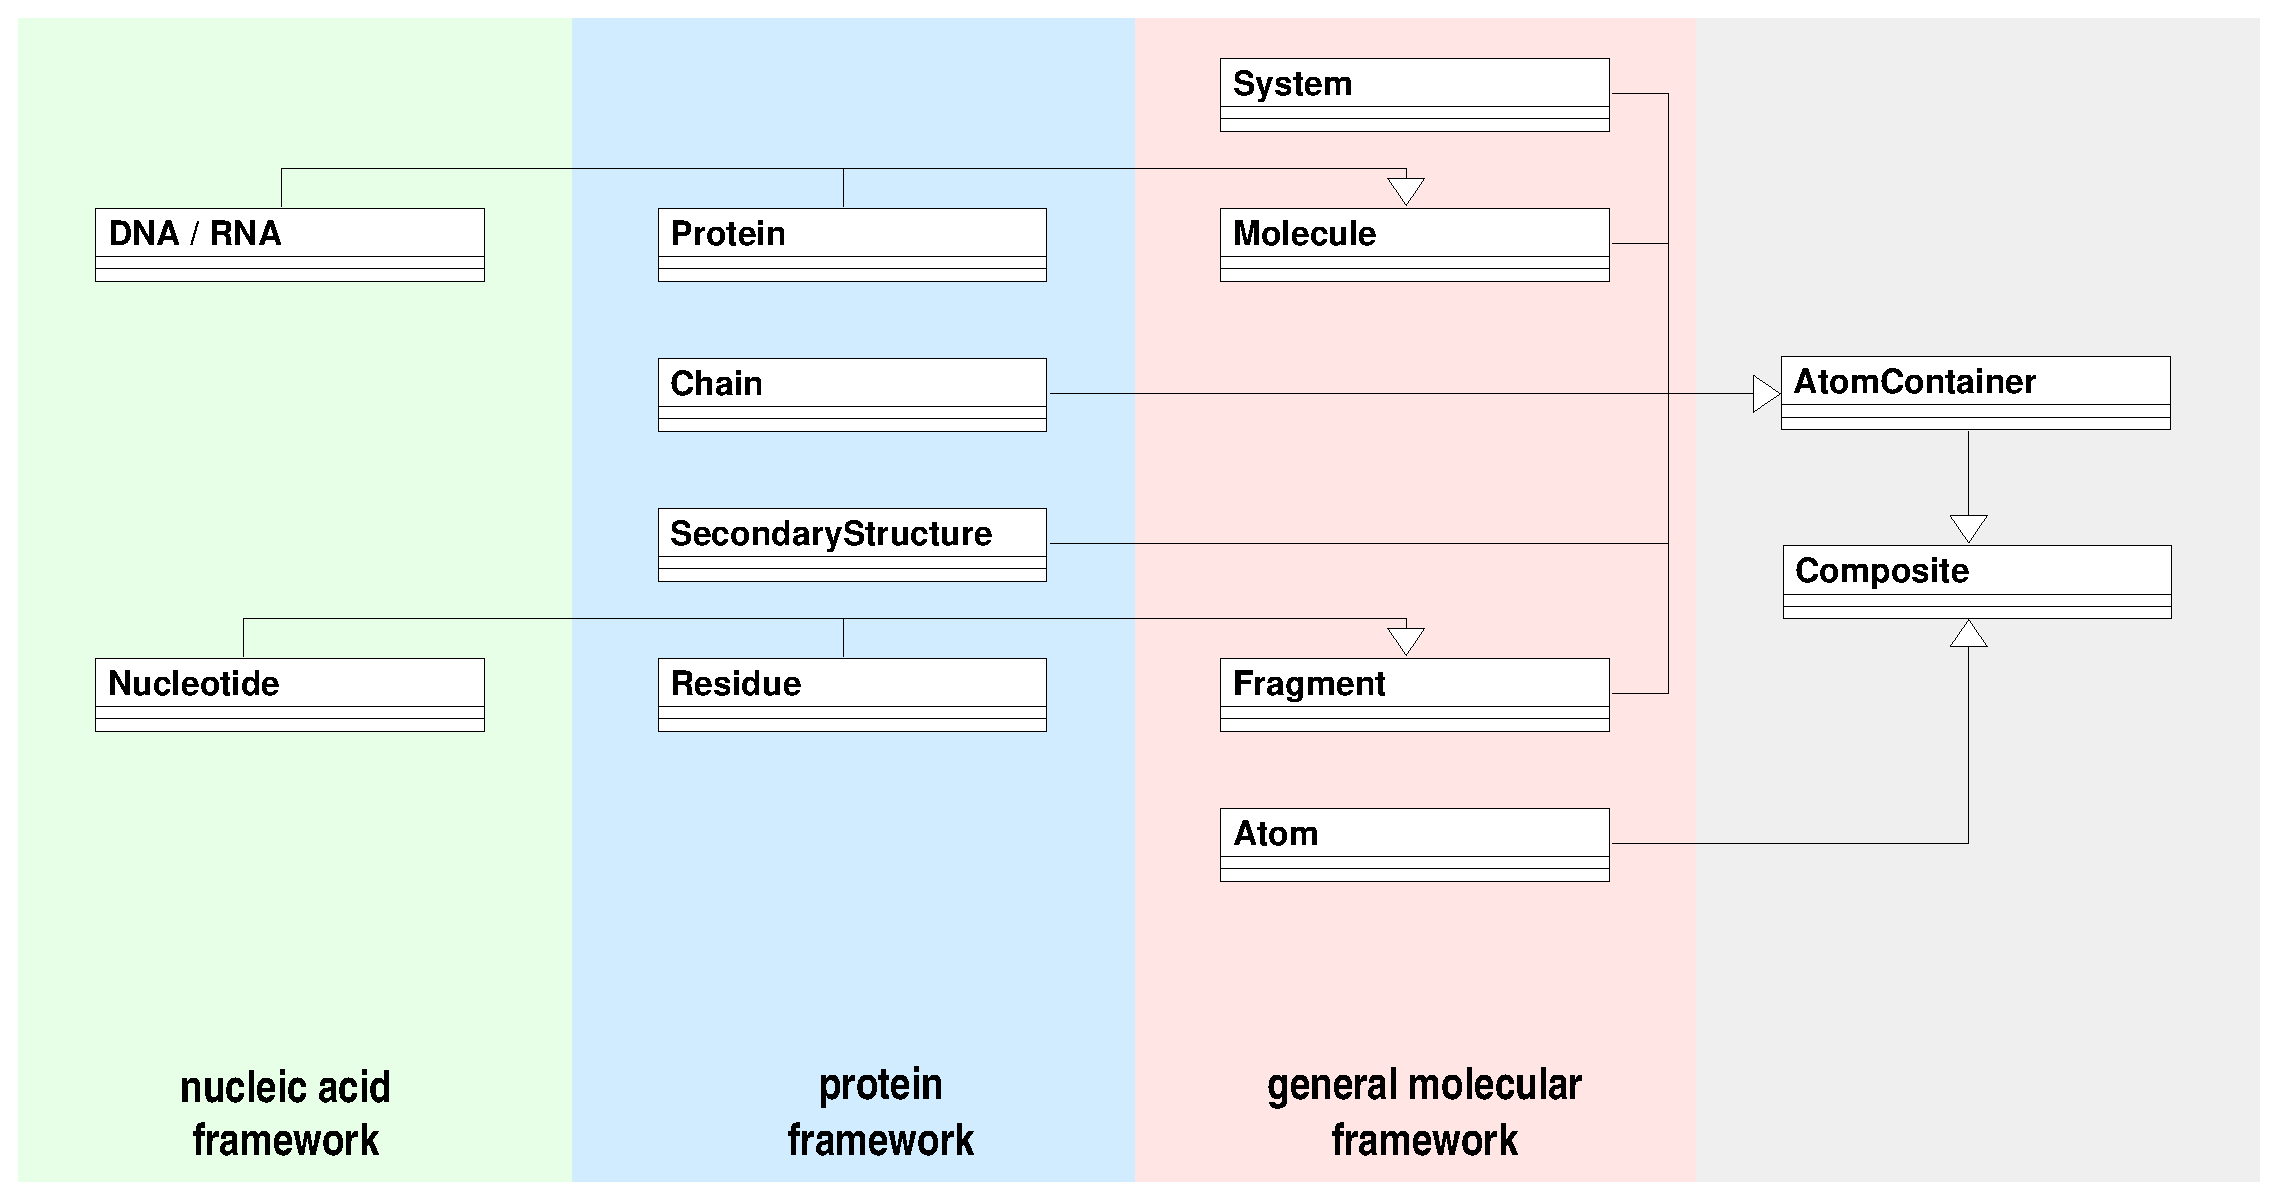
\includegraphics[width=\textwidth]{kernel-data-structures}
  \caption{The BALL kernel classes consist of three main frameworks: the
           molecular framework, the protein framework, and the nucleic acid
           framework.}
  \label{figure:kernel-frameworks}
\end{figure}


\subsection{Molecular Framework}
\label{section:molecularframework}

The molecular framework contains the classes \class{System},
\class{Molecule}, \class{Fragment}, \class{Bond}, and \class{Atom}. 
Molecules can contain an arbitrary number of atoms or fragments. A fragment
can be used to define distinct groups in a molecule, \eg functional groups or
charge groups. Fragments can be nested, so you may want to define several
functional groups within one larger fragment in a molecule. The atoms are then
contained in the fragments. In contrast to other systems, the atoms of a
molecule are not necessarily connected to each other (or in graph-theoretical
terms: they do not have to represent a connected component of the graph
formed by atoms and bonds). Systems are nothing but collections of molecules.


\subsection{Protein Framework}
\label{section:proteinframework}

The protein framework is a specialization of the general molecular
framework and describes the structures encountered in proteins. Proteins are
(more or less) molecules, so \class{Protein} is a subclass of \class{Molecule}
and proteins can be handled like molecules and stored along with them in
systems. Proteins can often be decomposed into several chains. These chains in
turn can contain secondary structure elements, which then contain residues.
Residues usually describe the amino acids of a protein. The sequence
information of a protein is encoded implicitly in the order of the tree: it
can be obtained by reading all instances of \class{Residue} in the order they
are contained in a protein. So the protein, the chains, and secondary
structure elements should contain the residues in the correct order, from
N-terminal to C-terminal, if you construct them by hand. The first and last
residue of a chain are considered to be terminal (according to the member
function \member{Residue}{isTerminal}). This is also the reason why a protein
should always contain at least one chain. Secondary structure elements,
defined by \class{SecondaryStructure}, are optional. Wherever this information
is known (\eg when read from PDB files), instances of
\class{SecondaryStructure} are created to store it. Each secondary structure
element has a property (\eg helix, $\beta$-sheet) describing its type.


\subsection{Nucleic Acid Framework}
\label{section:nucleicacidframework}

The nucleic acid framework contains the classes \class{NucleicAcid}
and \class{Nucleotide} and is used to represent structures of nucleic acids.


\section{Kernel Iterators}
\label{section:iterators}

Iteration over kernel data structures is a key concept in BALL.
The BALL kernel iterators are STL-like iterators. Since most BALL kernel
classes are so-called {\em multi-containers}, \ie they can contain different
objects, we cannot use the typical STL {\tt begin()}/{\tt end()} methods.
For example, in a protein, you might not only want to iterate over all chains,
but also over all residues or all atoms contained therein. BALL offers
the methods \member{System}{beginChain()}/\member{System}{endChain()},
\member{System}{beginAtom()}/\member{System}{endAtom()}, and so on for all
kernel classes. Similarly, the iterators are not {\tt typedef}ed within the
class, but are independent classes, because an \class{AtomIterator} could be 
defined for any kernel class containing atoms. The only exception from that rule
is \class{Atom::BondIterator}, since an atom is the only container having
bonds.

We can use those iterators in an STL-like fashion

\begin{lstlisting}{}
  Molecule m = ...;
  AtomIterator ai;
  for (ai = m.beginAtom(); ai != m.endAtom(); ++ai)
  {
    ...
  }
\end{lstlisting}

\noindent but there is also a convenient shorthand: the \method{operator +}
for all iterators. In contrast to STL iterators, BALL iterators are tightly 
bound to their containers and are thus aware of the container's end.
The plus operator returns a boolean value determining the validity of the
operator. It will return {\bf false} as soon as the iterator reaches the
end of the container. So we can rewrite the above code as:

\begin{lstlisting}{}
  Molecule m = ...;
  AtomIterator ai(m.beginAtom());
  for (; +ai; ++ai)
  {
    ...
  }
\end{lstlisting}

\noindent 
There exist several variants of the kernel iterators: the standard
forward iterators (\eg \class{AtomIterator}) and reverse iterators
(\class{AtomReverseIterator}). For both, there are also {\tt const} versions of
these iterators, which are required when iterating over {\tt const}  instances
of kernel classes (\class{Atom\-Const\-Iterator},
\class{Atom\-Const\-Reverse\-Iterator}).
Iteration is possible for all kernel classes, if they can contain the
respective instances. So it is possible to iterate over all atoms in a
molecule, but it is not possible to iterate over all chains of a residue,
because \class{Residue} does not provide the {\tt beginChain}/{\tt endChain}
methods.

Analogously to the STL, iterators may be dereferenced using both the star 
operator \index{operator {\tt *}}, and the arrow operator: 
\index{operator {\tt <<}}

\begin{lstlisting}{}
  AtomIterator ai = molecule.beginAtom();
  cout << "first atom: " << (*ai).getName() 
       << " @ " << ai->getPosition() << std::endl;
\end{lstlisting}

